% BRED

\section{Introduction}

One of the central cellular processes underlying development is transcriptional regulation. 
Modelling the dynamics of gene regulation is therefore essential to better understand
why a cellular dynamic processes progresses through several steps,
and what goes wrong in the case of disease. 
Regulatory dynamics is classically studied using time series data \cite{bar-joseph_studyingmodellingdynamic_2012}. When dynamic processes progress asynchronously, such as in hematopoiesis, time series data are usually obtained by sorting different transition states and assessing bulk gene expression and transcription factor binding within the population \cite{novershtern_denselyinterconnectedtranscriptional_2011, may_dynamicanalysisgene_2013, jojic_identificationtranscriptionalregulators_2013, goode_dynamicgeneregulatory_2016}. Alternatively, time series data can also be generated by synchronising the dynamic process between cells. However, issues with time-resolution, heterogeneity and good \textit{in vivo} synchronisation models can often limit the predictive power of the dynamic models of gene regulation which can be constructed \cite{bar-joseph_studyingmodellingdynamic_2012}.

Network inference (NI) methods are computational tools which use large omics datasets to predict which genes are regulated by which transcription factors. While accuracy of the network of predicted regulatory interactions is lower in comparison to experimental validation techniques, NI methods offer an unbiased and high-throughput insight into the regulatory dynamics of a biological system.
The output of a network inference is thus a graph, where nodes represent genes and edges denote a regulatory interaction between a regulator and a target gene. Interactions have two properties: its regulatory strength (a positive real value) and its effect (promoting or repressing).

Several studies have highlighted how some regulatory interactions can be very dynamic while others show evidence of being static during consecutive developmental stages \cite{moignard_characterizationtranscriptionalnetworks_2013, pina_singlecellnetworkanalysis_2015}. 
Since regulatory interactions are context-dependent \cite{papp_genomewideanalysiscontextdependence_2005}, attempting to create an accurate model of those processes by inferring a static regulatory network may have limited relevance.
Case-wise NI methods\footnote{Case-wise NI is sometimes also called sample-specific NI or case-specific NI.} avoid predicting a static GRN and instead infer one GRN per cell (or per sample, for bulk omics data).

In order to compute a case-wise GRN for a single sample, Kuijjer et al. \cite{kuijjer_estimatingsamplespecificregulatory_2019} and Liu et al. \cite{liu_personalizedcharacterizationdiseases_2016} employ similar strategies, namely by computing the difference of computing a static GRN for all the cases, and computing a static GRN for all the cases minus one. Since this procedure needs to be repeated for every case in the dataset, and because NI methods are already amongst the most computationally intensive analyses to perform on omics data, this methodology is not applicable for large omics datasets.
Another case-wise NI method, SCENIC \cite{aibar_scenicsinglecellregulatory_2017} infers case-wise GRNs by first inferring a static GRN using GENIE3 \cite{huynh-thu_inferringregulatorynetworks_2010}. GENIE3 is a static NI method which uses Random Forests (RFs) \cite{breiman_randomforests_2001} variable importance scores to prioritise candidate regulators for a particular target gene. SCENIC then post-processes the static GRN to determine whether an interaction is enriched for particular cases, resulting in a case-wise GRN. 

Thus, while several case-wise NI methods have already been proposed, their implementation consisted of post-processing a static GRN to arrive at a case-wise GRN. As such, these methods will most likely recover the interactions that are prevalent in the whole population, and will miss interactions that are specific to only a sub-population.

In this work, we introduce \texttt{bred}, the first 'true' case-wise NI method. It uses a modified version of the RF variable importance scores used by GENIE3 and SCENIC to compute importance values for each profile and each interaction separately, as well as predict the effect of each interaction (activating or repressing). We generate case-wise GRNs -- or case-wise regulomes -- for 14'963 profiles from The Cancer Genome Atlas (TCGA) \cite{weinstein_cancergenomeatlas_2013}, resulting in 6'464'915 predicted case-wise interactions.
We analyse these case-wise regulomes by clustering them and detecting highly activated interactions.

\section{Results}
At the time of writing, the TCGA database contains 14'963 profiles from 44 different cancer entities. We used the \texttt{bred} algorithm to infer case-wise regulomes for each of these profiles. In total, we detected 73'140 unique interactions and, on average, 7'231 active interactions per profile. Dimensionality reduction and clustering of the case-wise regulome data provides a visual overview of the different subpopulations (Figure~\ref{fig:tcga_dimred}).

\begin{figure}[htb!]
	\centering
	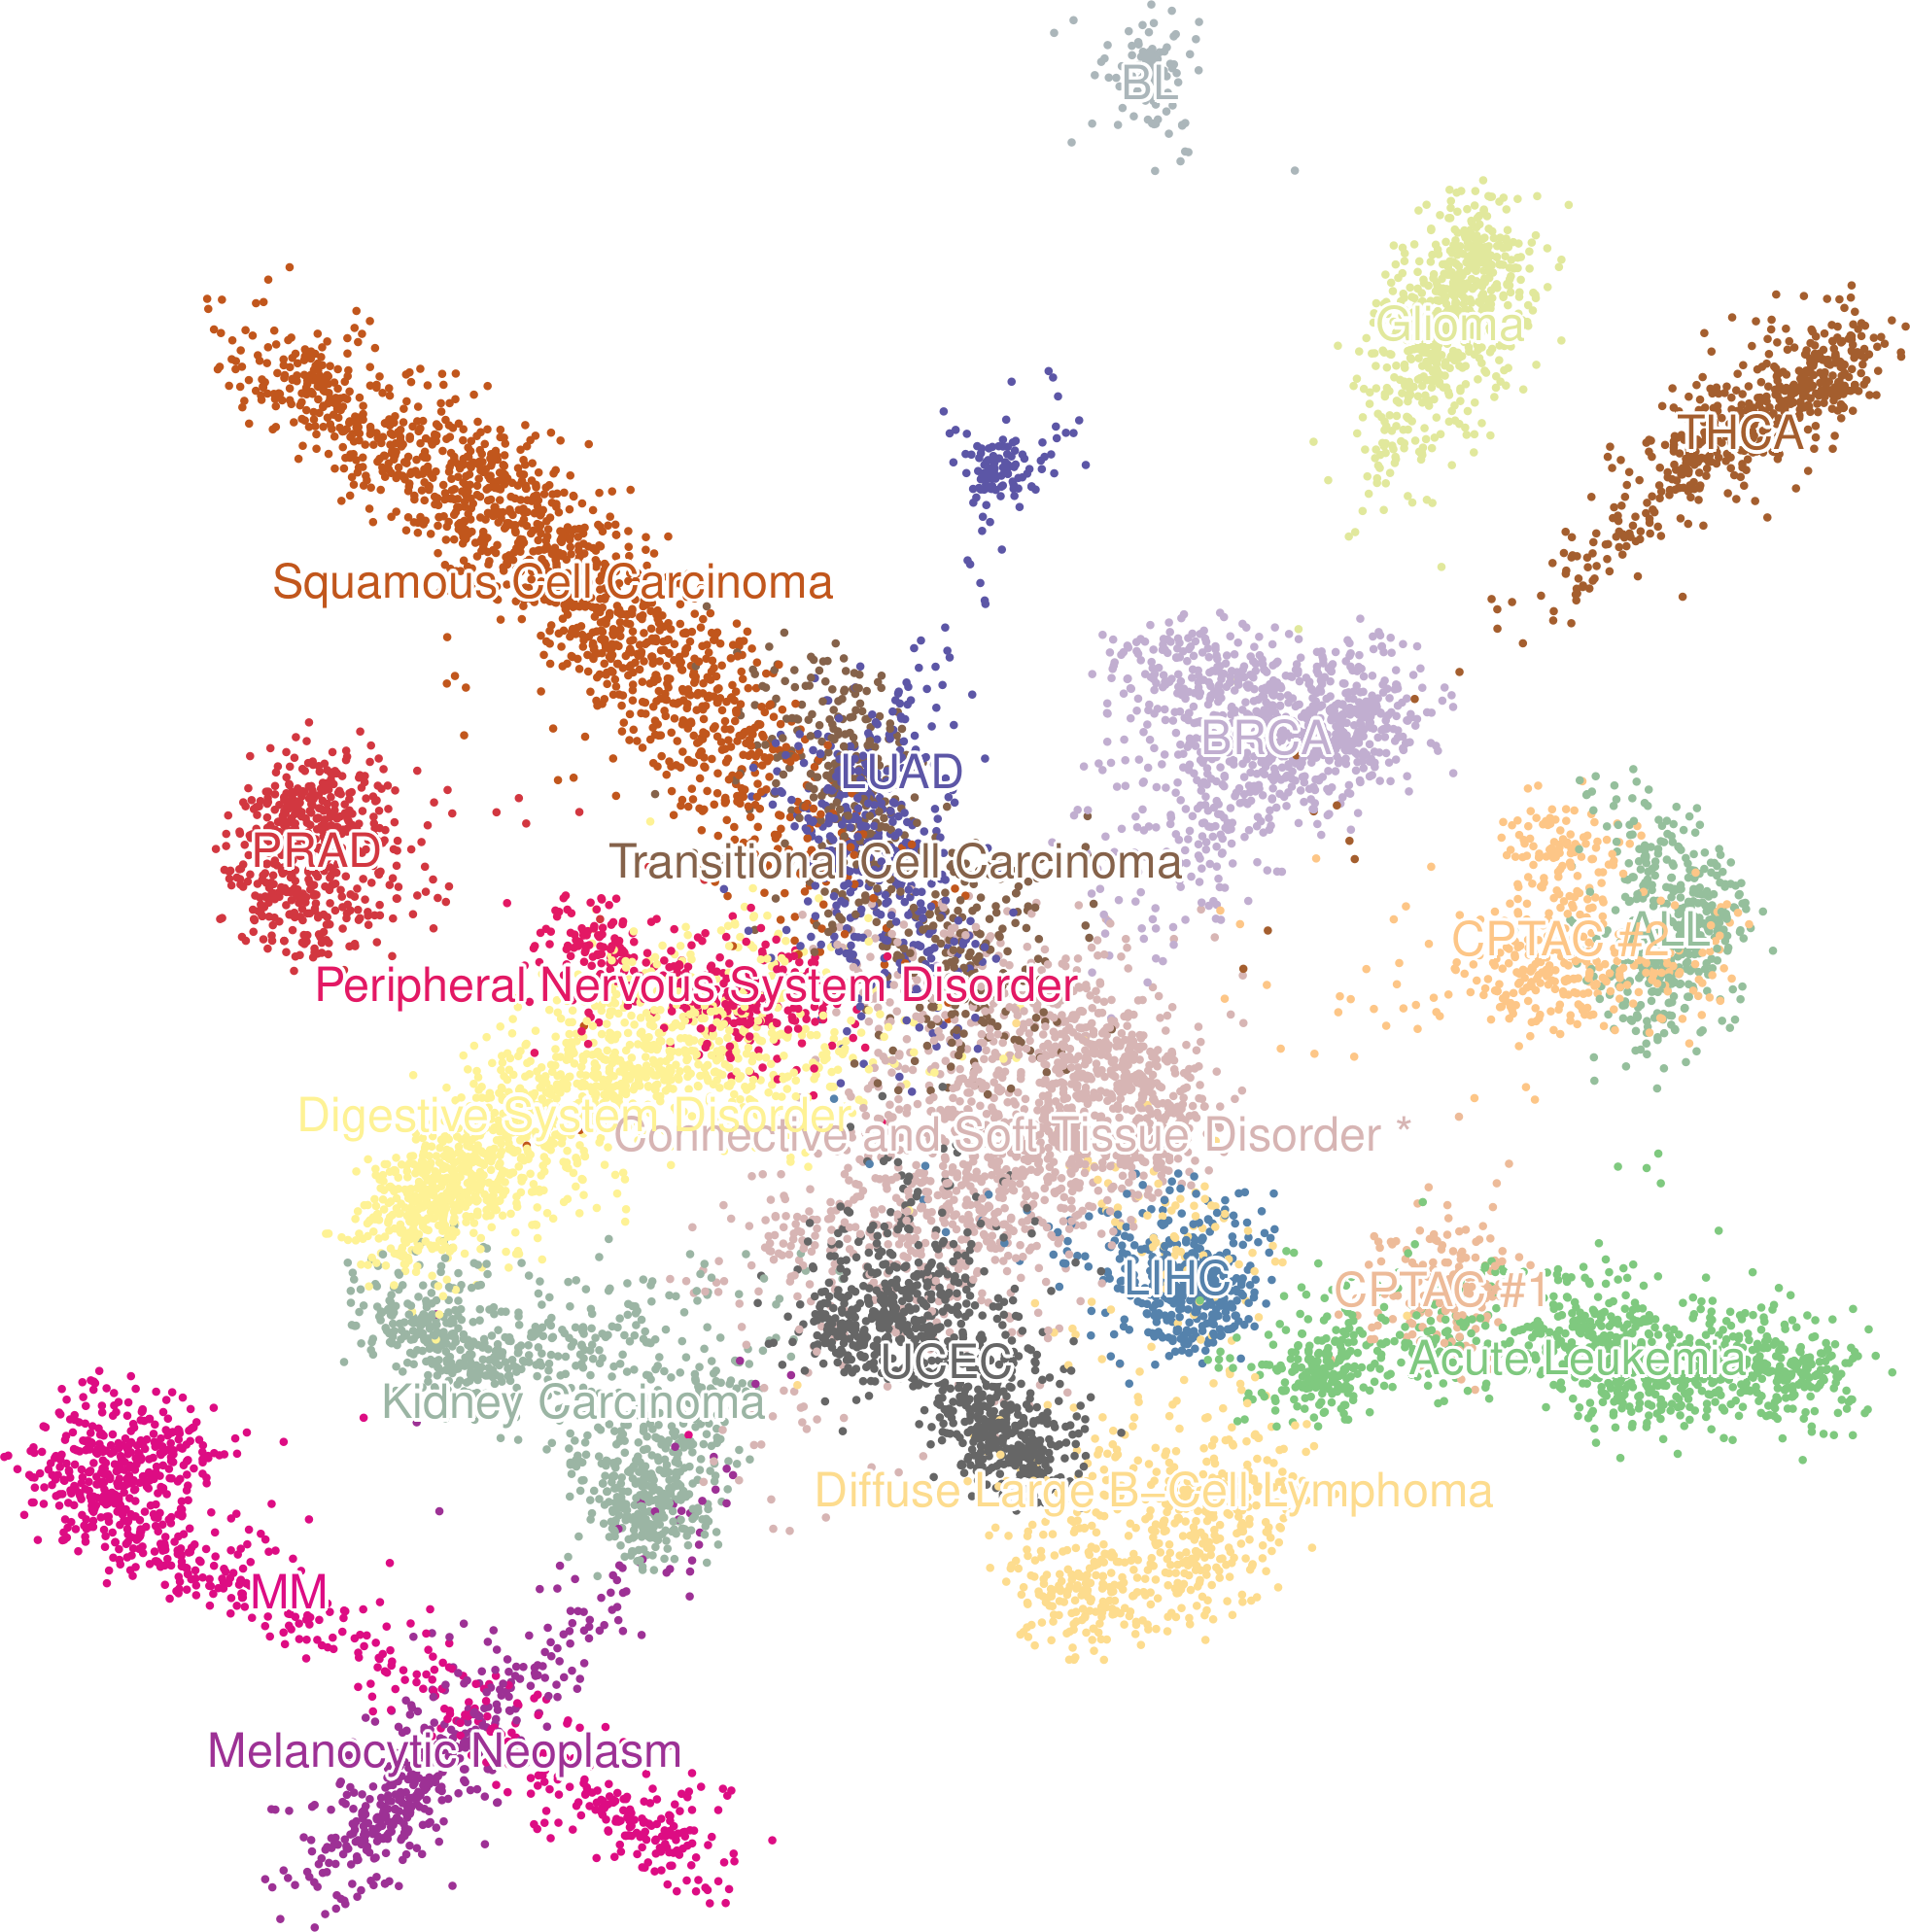
\includegraphics[width=.6\linewidth]{fig/tcga/plot_fr_cropped.png}
	\caption{
		\textbf{Visualisation of 14'963 case-wise regulomes of cancer profiles from The Cancer Genome Atlas project.} 
		Dimensionality reduction of the case-wise regulomes was performed by applying Fruchterman-Reingold \cite{fruchterman_graphdrawingforcedirected_1991} on the $k$-nearest-neighbour graph ($k=100$) of highly similar regulomes (Spearman correlation). The samples were clustered with Louvain clustering \cite{blondel_fastunfoldingcommunities_2008} and each cluster was assigned an ontology term from the NCI thesaurus ontology \cite{sioutos_ncithesaurussemantic_2007} which best fits the sample in the cluster. Clusters for which the term has a positive predictive value (PPV) lower than 0.5 are marked with an asterisk (*). More detailed information on the enrichment of particular terms or metadata for each of the clusters can be found in Figures~\ref{fig:cluslab1}--\ref{fig:cluslab7}.
	}
	\label{fig:tcga_dimred}
\end{figure}

For each cluster, we computed the average importance of each interaction. Retaining the 100 strongest interactions (Figure~\ref{fig:tcga_network}) shows that different cancer entities have vastly different regulomes, yet often have shared regulators and interactions (Table~\ref{tab:oncogenes}).

\begin{figure}[htb!]
	\centering
	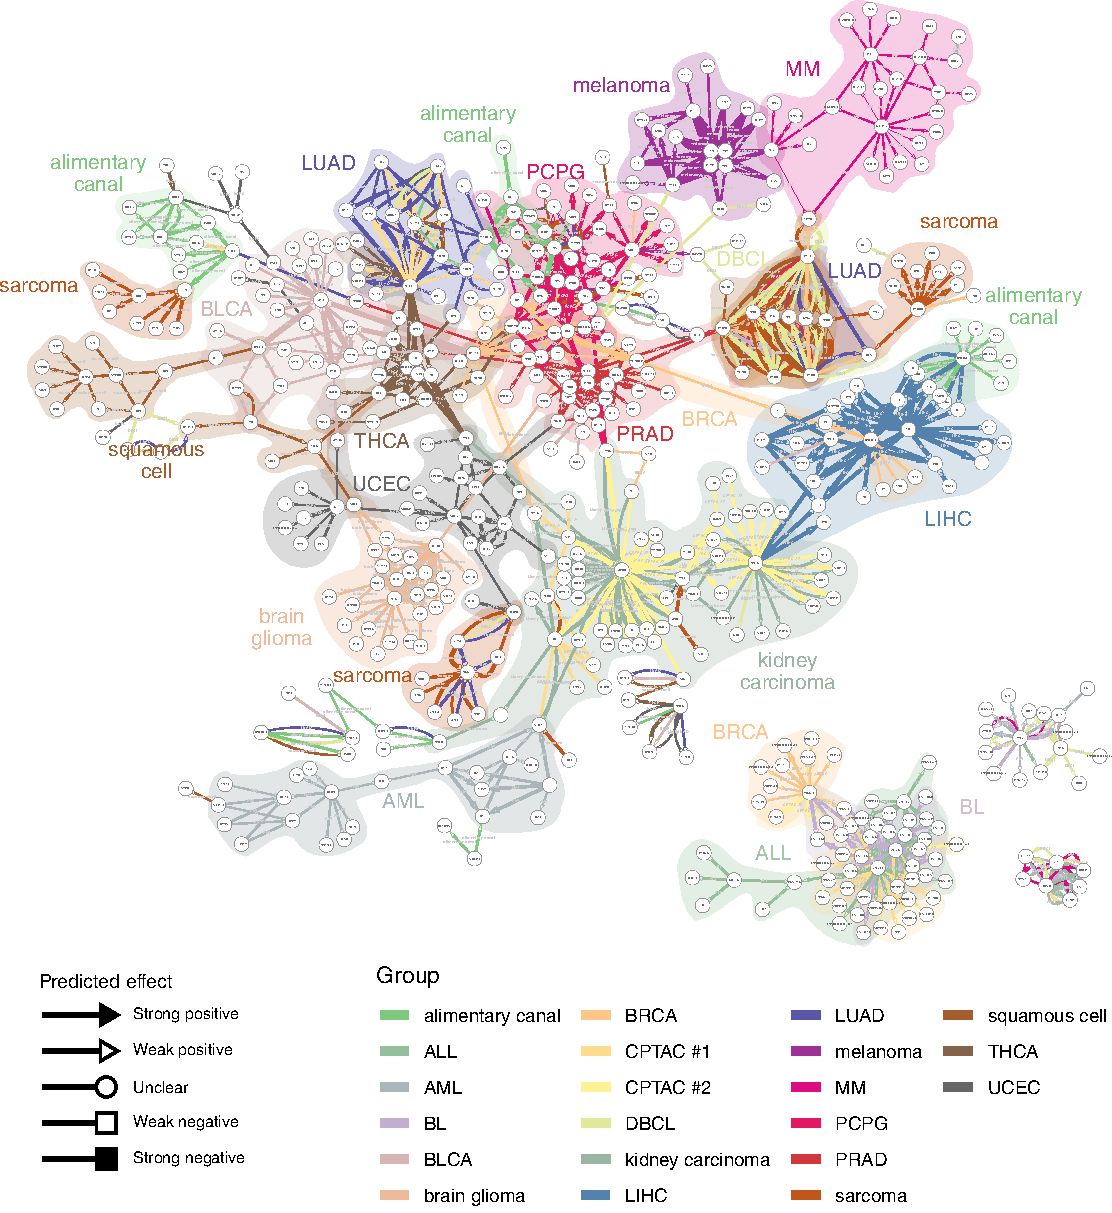
\includegraphics[width=.85\linewidth]{fig/tcga/grouped_interactions.pdf}
	\caption{
		\textbf{Visualisation of the strongest interactions per cluster} shows both pathways distinct to particular cancer entities as well as pathways common to multiple cancer entities.
	}
	\label{fig:tcga_network}
\end{figure}

Performing a more in-depth analysis of particular clusters can reveal distinct sub-populations within. For example, when comparing samples of normal and healthy tissue within breast carcinoma (Figure~\ref{fig:zoom17}), a significant number if interactions are predicted to have been turned off (top), while others have been turned on (middle, bottom). Similar observations can be made for other clusters, such as for melanocytic neoplasm (Figure~\ref{fig:zoom9}) and kidney carcinoma (Figure~\ref{fig:zoom12}).

\begin{figure}[htb!]
	\centering
	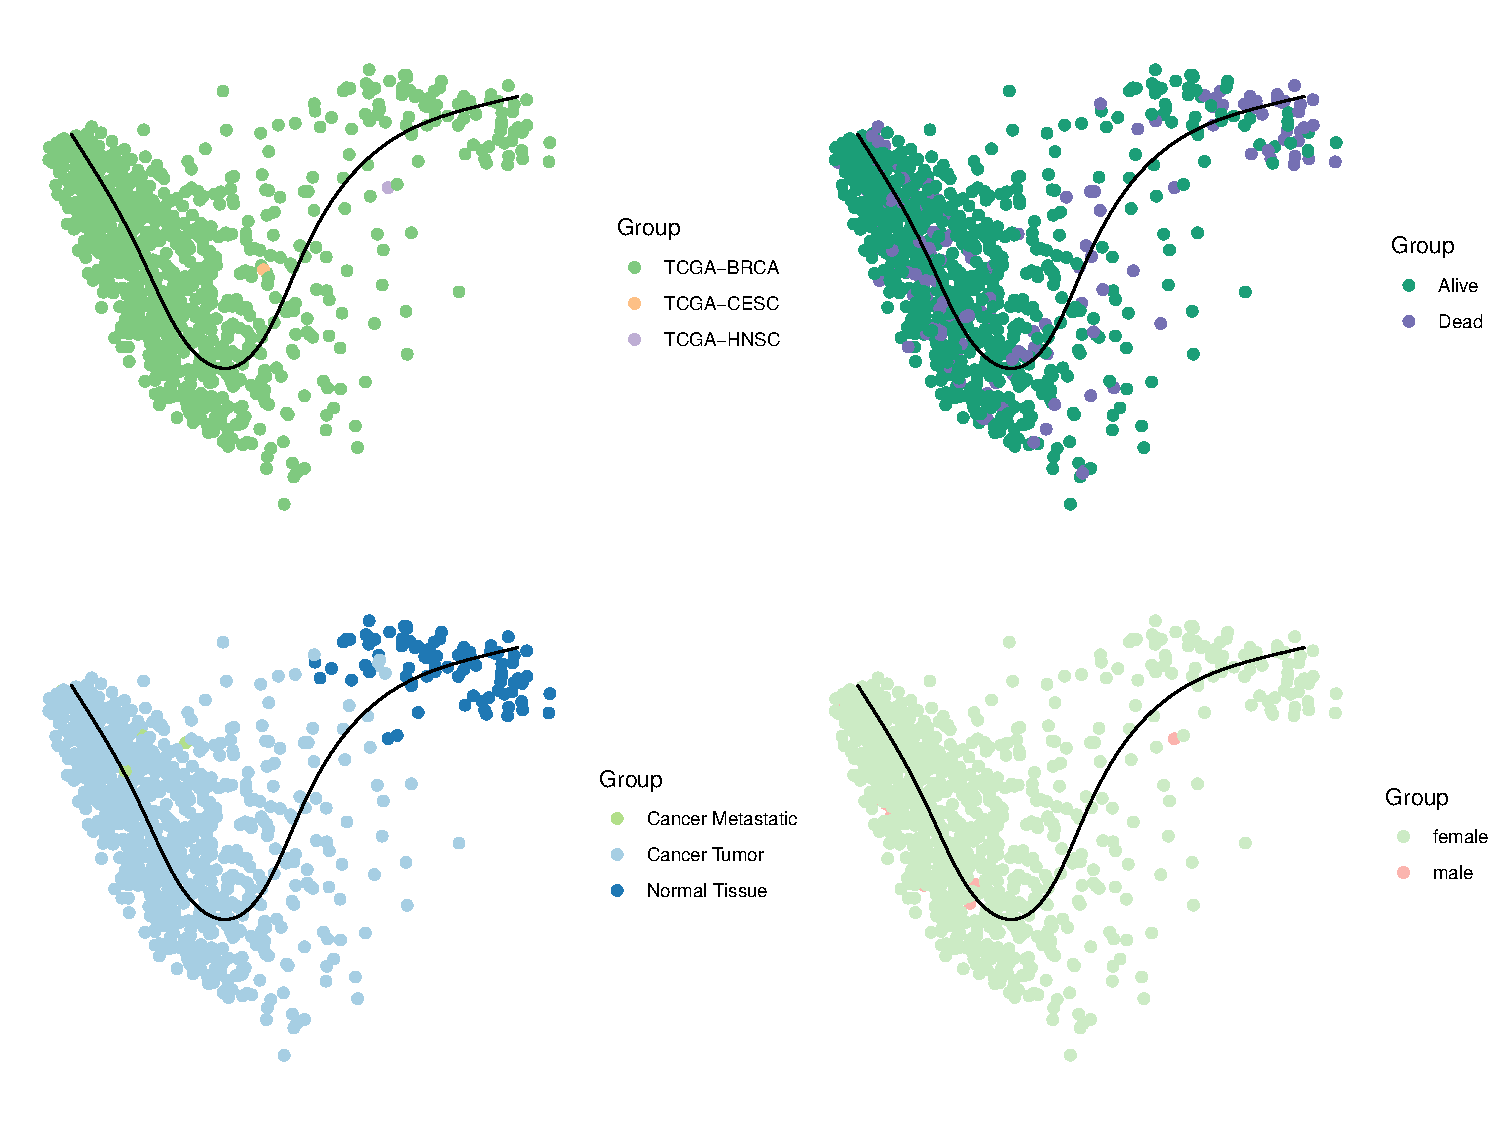
\includegraphics[width=.7\linewidth]{fig/tcga/zoom_cluster17_brca_plot.pdf}
	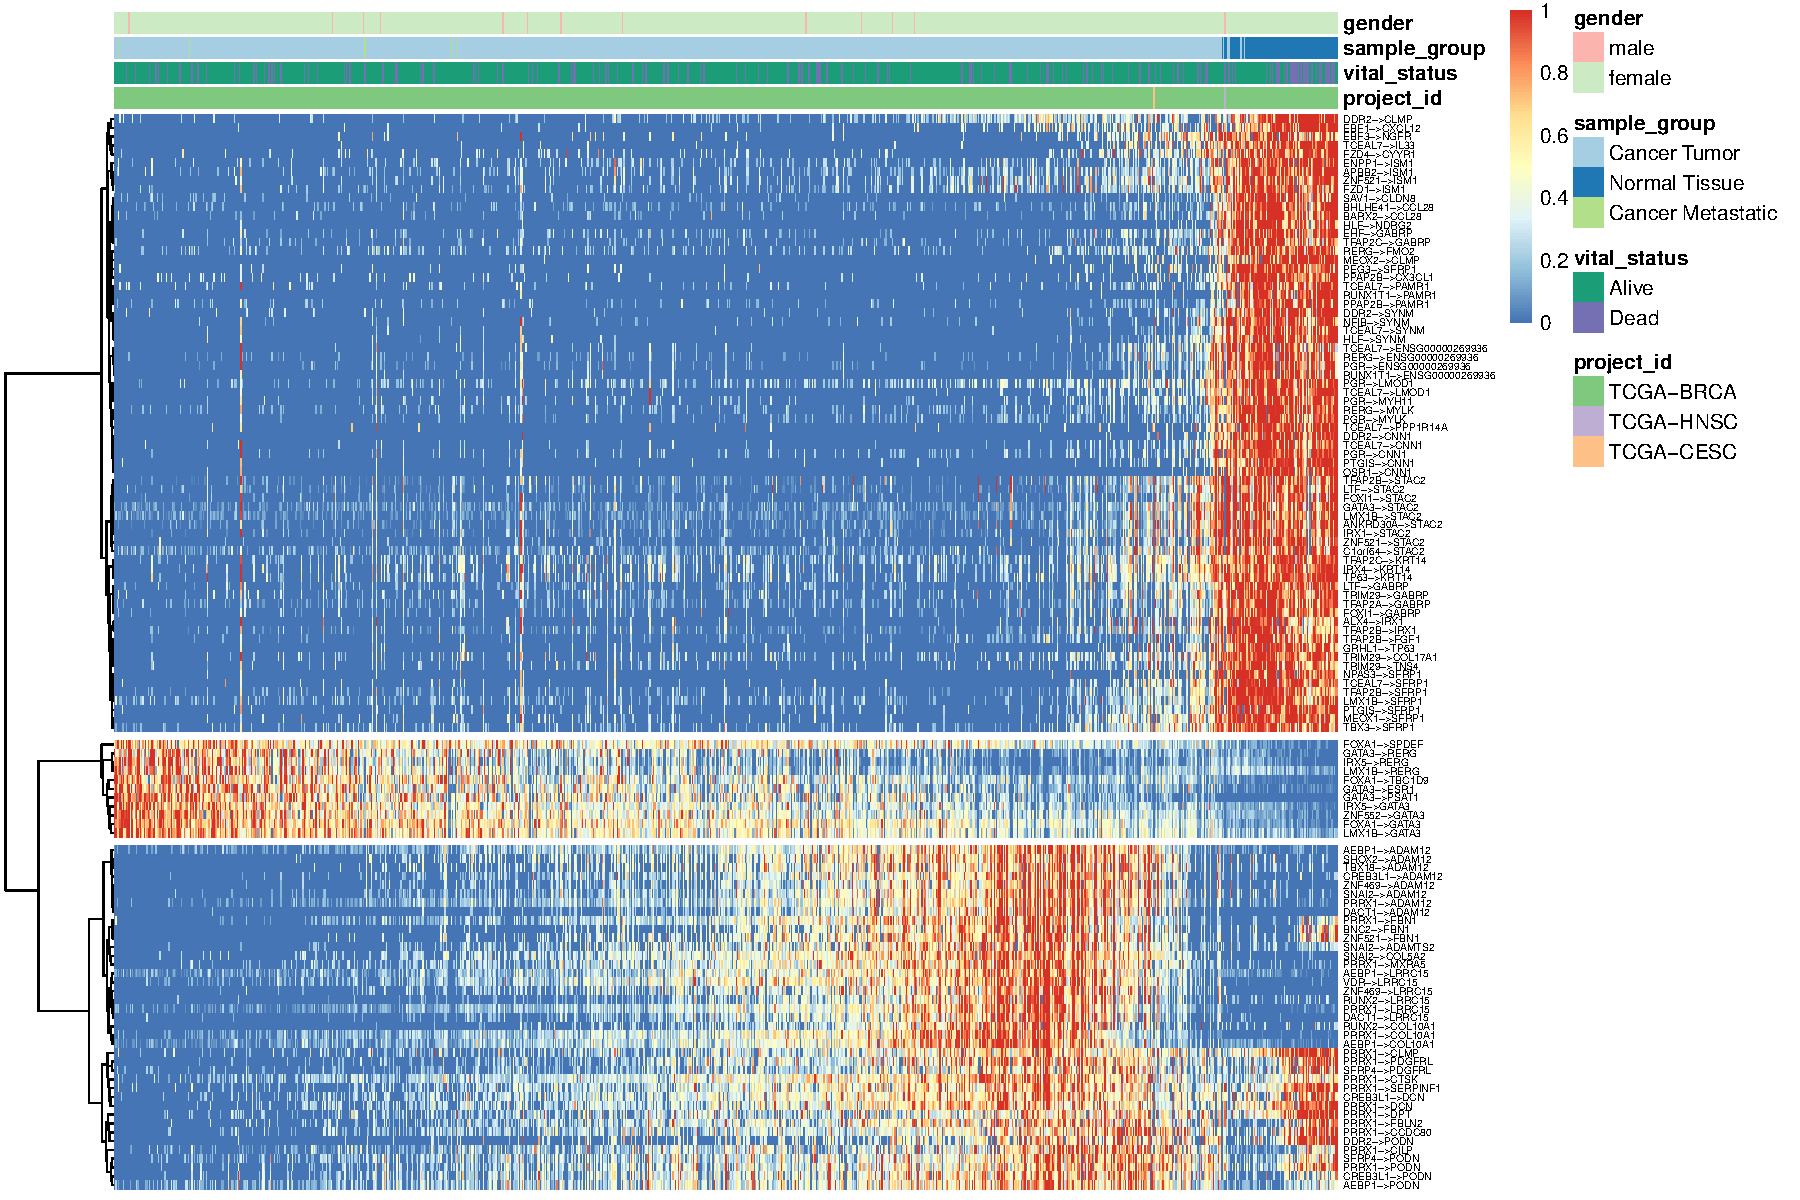
\includegraphics[width=.7\linewidth]{fig/tcga/zoom_cluster17_brca_heatmap.pdf}
	\caption{
		\textbf{In-depth view of cluster 17, breast carcinoma.} 
		\textbf{Top:} A dimensionality reduction of the samples, coloured according to multiple sources of meta-data. 
		\textbf{Bottom:} The samples were ordered linearly with SCORPIUS (see trajectory in \textbf{Top}) in order to visualise regulome activity in the form of a heatmap.
	}
	\label{fig:zoom17}
\end{figure}


\section{Discussion}

The \texttt{bred} algorithm is a novel approach for directly computing case-wise regulomes for single-cell omics and bulk omics profiles alike. We used \texttt{bred} to infer case-wise regulomes for 14'963 cancer profiles from The Cancer Genome Atlas project. Analysing the results using common omics algorithms (dimensionality reduction, clustering, enrichment) has shown that regulatory interactions are often specific to particular cancer types, but can also be shared between several cancer types. Ultimately, this analysis has resulted in a list of candidate oncogenic genes and interactions per cancer type, though further analysis and validation is required to confirm their oncogenicity.

Future perspectives include applying it on single-cell omics data (e.g. from Tabula Muris \cite{schaum_singlecelltranscriptomics20_2018}) and benchmarking the algorithm against \textit{in silico} datasets (e.g. produced by \texttt{dyngen} \cite{cannoodt_dyngenbenchmarkingsilico_2019}).

\section{Methods}

\subsection{Inferring case-wise regulomes}
The task of inferring a static GRN (Figure~\ref{fig:simplify}A) can be reduced to a simpler problem, namely: for every target $T$, predict which of the potential regulators $R_i$ regulate $T$ (Figure~\ref{fig:simplify}B). This simplification allowed GENIE3 \cite{huynh-thu_inferringregulatorynetworks_2010} to use Random Forest's \cite{breiman_randomforests_2001} feature importance scores for inferring GRNs. Namely, a Random Forest is trained to predict the expression of a target gene of interest from the expression of potential regulators. The resulting Random Forest inherently allows to extract a feature importance score by observing the effect of each regulator in making a good prediction for the target expression. As in GENIE3, the target expression is first scaled to normalise feature importance scores across different targets.

\begin{figure}[htb!]
	\centering
	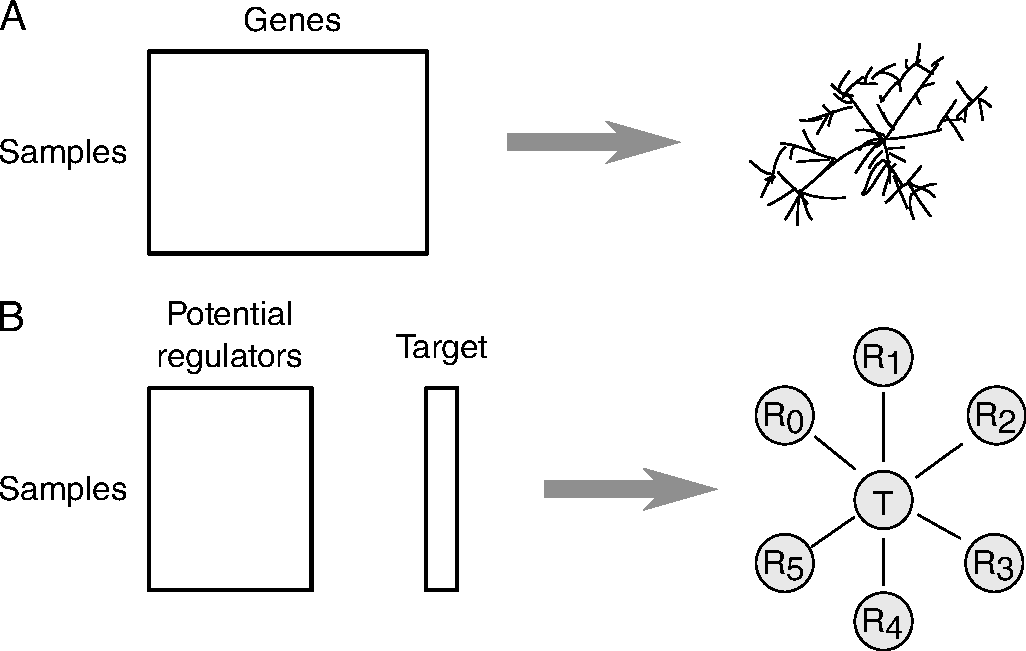
\includegraphics[width=.6\linewidth]{fig/methodology/simplify.pdf} 
	\caption{
		\textbf{A:} Inferring a gene regulatory network from an omics dataset can be reduced to a simpler problem. 
		\textbf{B:} Given the expression of a target of interest and a set of potential regulators, predict which regulators regulate the target gene.
	}
	\label{fig:simplify}
\end{figure}

We make the same simplification in order to build case-wise GRNs, also using Random Forests to compute the feature importance scores. A Random Forest consists of $K$ trees, each of which produces feature importance scores, and the feature importance scores of a forest is simply the mean feature importance scores of each of the trees. 

Computing the case-wise feature importances of a tree consists of the following 8 steps (Figure~\ref{fig:fimp}).
The 'randomness' of a Random Forest is due to only using a subset of the samples in the dataset in order to build a single decision tree. The samples are split into two groups, the 'in-bag' data and the 'out-of-bag' data (Figure~\ref{fig:fimp}A). A decision tree \cite{breiman_classificationregressiontrees_1984} is trained on the in-bag expression of the potential regulators in trying to predict the in-bag target gene expression (Figure~\ref{fig:fimp}B). The target expression of the out-of-bag samples is predicted using the decision tree (Figure~\ref{fig:fimp}C), and the squared error between the real and target expression is computed (Figure~\ref{fig:fimp}D). For each sample in the out-of-bag set, this vector represents how well the decision tree was able to predict the expression of the target gene.

The next few steps are repeated for every potential regulator $R_i$. Within the out-of-bag samples, the expression of $R_i$ is randomly shuffled. The target expression of the out-of-bag samples is again calculated (Figure~\ref{fig:fimp}F), as well as the squared error between the real target expression and the predicted expression is calculated (Figure~\ref{fig:fimp}G). The importance of regulator $R_i$ for an out-of-bag sample $S_j$ is defined as the increase in squared error between the predicted target expression and the real target expression, after perturbing the expression of $R_i$ (Figure~\ref{fig:fimp}H). 

Steps F-G are repeated for every potential regulator $R_i$. By aggregating all of the feature importance scores over all the samples, regulators and targets, we obtain an $M$-by-$N$-by-$P$ tensor\footnote{This is the origin of the name of the method, "\texttt{bred}".}. 

A moderately-sized dataset could contain $M=10'000$ samples, $N=2'000$ regulators, and $P=10'000$ target genes. Due to memory constrains, only interactions with an average importance value (across all samples) higher than a minimum threshold are retained.

\begin{figure}[htb!]
	\centering
	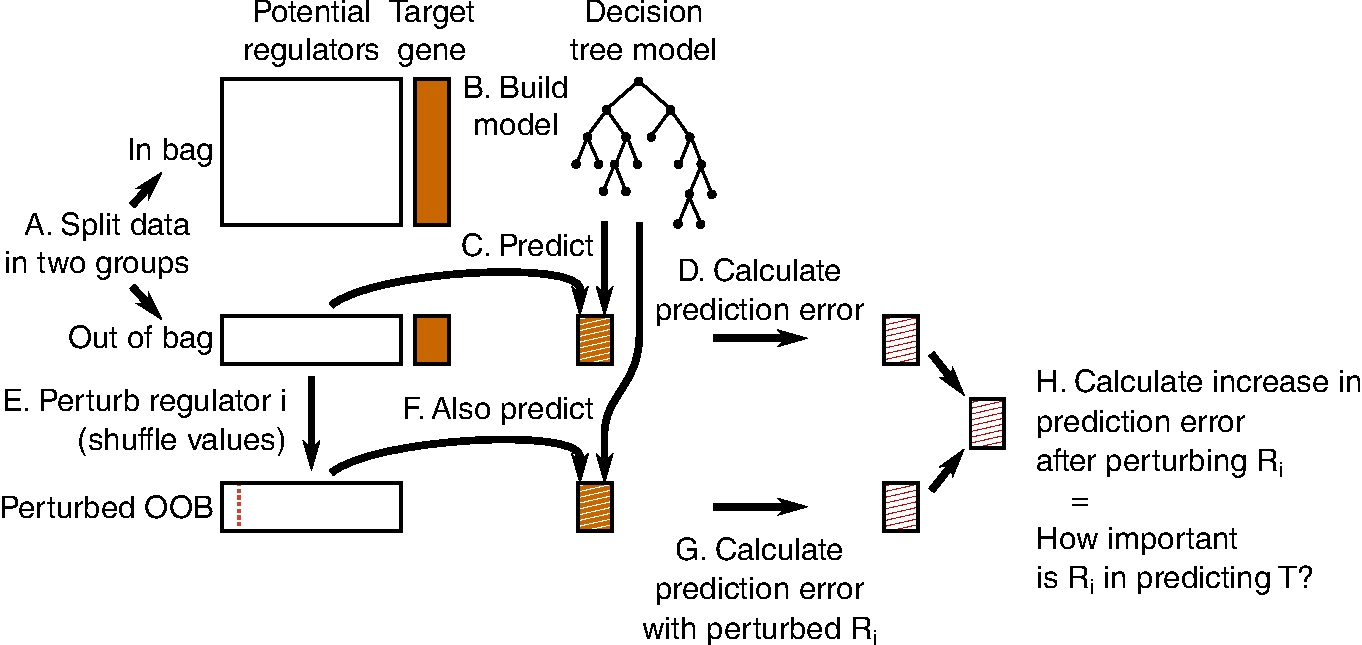
\includegraphics[width=.9\linewidth]{fig/methodology/fimp.pdf} 
	\caption{
		\textbf{Calculating the feature importance score for one decision tree and one target consists of 8 distinct steps.}
		\textbf{A:} Randomly split the data into two groups, the in-bag data and the out-of-bag data.
		\textbf{B:} The in-bag data is used to train a decision tree to try to predict the expression of the target gene from the expression values of the regulators.
		\textbf{C:} The decision tree is used to predict the gene expression of the target gene of the out-of-bag samples.
		\textbf{D:} Sample-specific squared error values are computed.
		\textbf{E:} Repeat steps E-H for every regulator $R_i$. Perturb the expression of regulator $R_i$ in the out-of-bag samples.
		\textbf{F:} Again predict the gene expression of the target gene with the perturbed expression values.
		\textbf{G:} Again compute the sample-specific squared error values.
		\textbf{H:} The difference between the prediction error on the perturbed dataset versus the prediction error on the unperturbed is the importance in $R_i$ in predicting $T$ 
	}
	\label{fig:fimp}
\end{figure}

To compute the case-wise GRNs, we implemented the abovementioned methodology in C++ in a modified version of the \texttt{ranger} R/C++ package \cite{wright_rangerfastimplementation_2017}.

\subsection{Predicting the effect of an interaction}
To predict the effect of a potential regulator $R_i$ on a target gene $T$ for a given tree, the Pearson correlation is calculated between the difference in regulator expression (before and after shuffling the values), and the difference in target expression prediction. 

\begin{align*}
  \text{effect}(R_i \rightarrow T) & = \text{cor}(x, y), \\
  \text{with } x & = \text{expr\_shuffled}[:,R_i] - \text{expr}[:,R_i], \\
  \text{and } y & = \text{predict}(\text{tree}, \text{expr\_shuffled}) - \text{predict}(\text{tree}, \text{expr}).
\end{align*}

The Pearson correlation between two variables $x$ and $y$ is usually defined as shown in Equation~\ref{eqn:pearson1}. Computing $r_{xy}$ for each (regulator, target) pairs, across all trees, would require storing large amounts of data.

\begin{equation}\label{eqn:pearson1}
	r_{xy} = \frac{\sum^n_{i=1} (x_i - \bar{x}) \times (y_i - \bar{y})}{\sqrt{\sum^n_{i=1}(x_i - \bar{x})^2}\times\sqrt{\sum^n_{i=1}(y_i - \bar{y})^2}}
\end{equation} 

However, by rearranging the formula, it can be defined as Equation~\ref{eqn:pearson2}.

\begin{equation}\label{eqn:pearson2}
r_{xy} = \frac{\sum(x_i \times y_i) - \sum x \times \sum y / n}{\sqrt{(\sum x_i^2 - (\sum x)^2 / n)} \times \sqrt{(\sum y_i^2 - (\sum y)^2 / n)}}
\end{equation}

For every regulator $R_i$ during a perturbation in a given tree, only 6 values need to be stored, namely $A = \sum x_i$, $B = \sum y_i$, $C = n$, $D = \sum{x_i \times y_i}$, $E = \sum{x_i \times x_i}$, and $F = \sum{y_i \times y_i}$.

For every (regulator, target) pair, these values are summed, and the $r_{xy}$ is calculated as shown in Equation~\ref{eqn:pearson3}.

\begin{equation}\label{eqn:pearson3}
r_{xy} = \frac{D - A \times B / C}{\sqrt{(E - A^2 / C)} \times \sqrt{(F - B^2 / C)}}
\end{equation}

The following cutoffs were used to determine the effect. 

\begin{itemize}
	\item Strong negative: $r_{xy} < -0.4$
  \item Weak negative: $-0.4 \leq r_{xy} < -0.2$
  \item Unclear: $-0.2 \leq r_{xy} \leq 0.2$
  \item Weak positive: $0.2 < r_{xy} \leq 0.4$
  \item Strong positive: $0.4 < r_{xy}$
\end{itemize} 

\subsection{Clustering of case-wise GRNs}
To perform downstream analysis on the cases, first a $k$-nearest neighbour ($k$NN) graph of the cases is computed.
In order for the $k$NN graph to better emphasise similarities in GRNs rather than absolute euclidean distances, we first reduce the dimensionality of the case-by-interaction matrix to case-by-20 matrix using Landmark Multi-Dimensional Scaling \cite{lee_landmarkmdsensemble_2009} with a Spearman rank distance metric.  

Next, KD-trees are used to calculate the $k$NN graph efficiently. The cases in the dataset are visualised and clusted using the Fruchterman-Reingold \cite{fruchterman_graphdrawingforcedirected_1991} and Louvain clustering \cite{blondel_fastunfoldingcommunities_2008}, respectively.

The following R packages provided implementations for each of these algorithms: lmds, RANN, igraph \cite{csardi_igraphsoftwarepackage_2006}.

% TODO: describe cluster relabelling, see figures fig:cluslab

\subsection{Visualising clustered GRNs}
After Louvain clustering, the interactions of the 50 interactions with highest mean importance per cluster are retained. These interactions are visualised in Cytoscape \cite{shannon_cytoscapesoftwareenvironment_2003}, in which nodes depict genes, edges depict predicted regulatory interactions, coloured according to which cluster they are predicted for. The shape of the arrow denotes the predicted effect of the regulatory interaction.

%\subsection{Data from the Tabula Muris project}
%
%\subsection{Data from The Cancer Genome Atlas project}

\section{Supplementary information}


\begin{table}[H]
	\scriptsize
	\caption{\textbf{Prioritisation of genes, ranked according to page-rank value.} The majority of these genes are already known to be involved in oncogenesis (data not shown).} \label{tab:oncogenes}
	\begin{tabularx}{\linewidth}{XX}
		\hline
		Cluster name & Top 4 genes, page rank \\
		\hline\hline
		Acute Leukemia & HSPA1A, HSPA1B, HOXA10, HOXA9 \\
		ALL & DDX3Y, XIST, RN7SL128P, TXLNGY \\
		BL & KIAA0226L, XIST, TCL1A, NUGGC \\
		BRCA & LINC00993, IRX5, ATP8A2P1, ENSG00000234918 \\
		Connective and Soft Tissue Disorder * & HOXA11, HOXC9, HOXA10, HOXC10 \\
		CPTAC \#1 & SLC22A2, CUBN, XIST, UMOD \\
		CPTAC \#2 & RN7SL752P, SCARNA13, XIST, RNY1 \\
		Diffuse Large B-Cell Lymphoma & PLA2G2D, ENSG00000224137, CCL25, MS4A1 \\
		Digestive System Disorder & MEP1A, LGALS4, MUC13, CDX1 \\
		Glioma & NCAN, GPM6A, MBP, OLIG2 \\
		Kidney Carcinoma & ACSM2A, SLC22A2, NAT8, UMOD \\
		LIHC & AGXT, ITIH3, ITIH1, HRG \\
		LUAD & SFTPA2, SFTPD, NAPSA, SFTA2 \\
		Melanocytic Neoplasm & MLANA, RPS4Y1, PMEL, TYR \\
		MM & CD96, GPRC5D, FGFR3, IGLV1-41 \\
		Peripheral Nervous System Disorder & TH, DBH, PENK, HAND2 \\
		PRAD & TRGC1, NKX3-1, ACPP, RPL7P16 \\
		Squamous Cell Carcinoma & TP63, SPRR2F, RPS4Y1, CDKN2B \\
		THCA & ENSG00000240237, TG, TPO, RPS4Y1 \\
		Transitional Cell Carcinoma & DHRS2, UPK2, PADI3, VGLL1 \\
		UCEC & DLX5, MSX1, HOXB5, HOXB8 \\
		\hline
		\	\end{tabularx}
\end{table}


\begin{figure}[H]
	\centering
	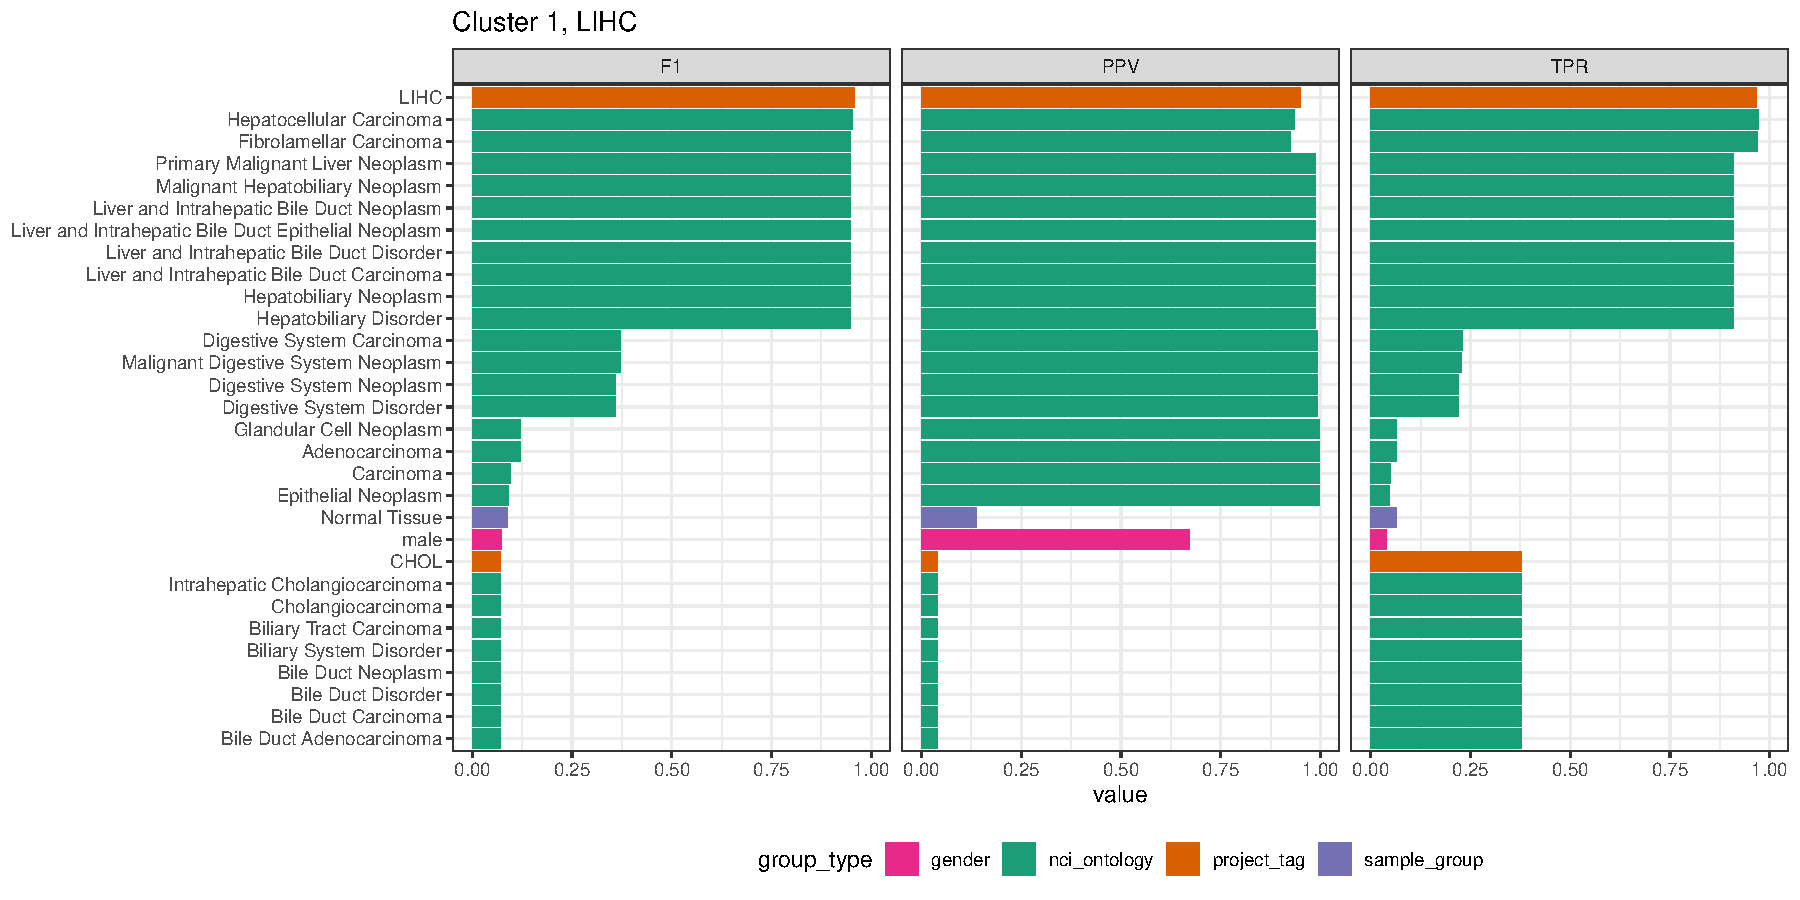
\includegraphics[width=.95\linewidth,page=1]{fig/tcga/cluster_labelling.pdf}
	\includegraphics[width=.95\linewidth,page=2]{fig/tcga/cluster_labelling.pdf}
	\includegraphics[width=.95\linewidth,page=3]{fig/tcga/cluster_labelling.pdf}
	\caption{
		\textbf{Prioritisation of NCI terms and other forms of meta-data used to annotate clusters 1--3.} Cluster 2 is mainly made up of disorders in female reproductive organs, and should have been labelled as such.
	}
	\label{fig:cluslab1}
\end{figure}

\begin{figure}[H]
	\centering
	\includegraphics[width=.95\linewidth,page=4]{fig/tcga/cluster_labelling.pdf}
	\includegraphics[width=.95\linewidth,page=5]{fig/tcga/cluster_labelling.pdf}
	\includegraphics[width=.95\linewidth,page=6]{fig/tcga/cluster_labelling.pdf}
	\caption{
		\textbf{Prioritisation of NCI terms and other forms of meta-data used to annotate clusters 4--6.} Cluster 5 is mainly made up of renal cell carcinoma, and should have been labelled as such. Cluster 6 is aptly named, but mainly consists of neuroblastoma (NB), pheochromocytoma (PC), and paraganglioma (PG) disorders.
	}
	\label{fig:cluslab2}
\end{figure}

\begin{figure}[H]
\centering
\includegraphics[width=.95\linewidth,page=7]{fig/tcga/cluster_labelling.pdf}
\includegraphics[width=.95\linewidth,page=8]{fig/tcga/cluster_labelling.pdf}
\includegraphics[width=.95\linewidth,page=9]{fig/tcga/cluster_labelling.pdf}
\caption{
	\textbf{Prioritisation of NCI terms and other forms of meta-data used to annotate clusters 7--9.} 
}
\label{fig:cluslab3}
\end{figure}

\begin{figure}[H]
\centering
\includegraphics[width=.95\linewidth,page=10]{fig/tcga/cluster_labelling.pdf}
\includegraphics[width=.95\linewidth,page=11]{fig/tcga/cluster_labelling.pdf}
\includegraphics[width=.95\linewidth,page=12]{fig/tcga/cluster_labelling.pdf}
\caption{
	\textbf{Prioritisation of NCI terms and other forms of meta-data used to annotate clusters 10--12.} 
	Cluster 11 contains mostly Lung Adenocarcinoma (LUAD), but also Lung Squamous Cell Carcinoma (LUSC), and thus should have been labelled Lung Carcinoma instead.
}
\label{fig:cluslab4}
\end{figure}


\begin{figure}[H]
	\centering
	\includegraphics[width=.95\linewidth,page=13]{fig/tcga/cluster_labelling.pdf}
	\includegraphics[width=.95\linewidth,page=14]{fig/tcga/cluster_labelling.pdf}
	\includegraphics[width=.95\linewidth,page=15]{fig/tcga/cluster_labelling.pdf}
	\caption{
		\textbf{Prioritisation of NCI terms and other forms of meta-data used to annotate clusters 13--15.} 
		Cluster 13 contains a mixture of cancer types, and should have been labelled 'Mixed'.
	}
	\label{fig:cluslab5}
\end{figure}

\begin{figure}[H]
	\centering
	\includegraphics[width=.95\linewidth,page=16]{fig/tcga/cluster_labelling.pdf}
	\includegraphics[width=.95\linewidth,page=17]{fig/tcga/cluster_labelling.pdf}
	\includegraphics[width=.95\linewidth,page=18]{fig/tcga/cluster_labelling.pdf}
	\caption{
		\textbf{Prioritisation of NCI terms and other forms of meta-data used to annotate clusters 16--18.} 
	}
	\label{fig:cluslab6}
\end{figure}

\begin{figure}[H]
	\centering
	\includegraphics[width=.95\linewidth,page=19]{fig/tcga/cluster_labelling.pdf}
	\includegraphics[width=.95\linewidth,page=20]{fig/tcga/cluster_labelling.pdf}
	\includegraphics[width=.95\linewidth,page=21]{fig/tcga/cluster_labelling.pdf}
	\caption{
		\textbf{Prioritisation of NCI terms and other forms of meta-data used to annotate clusters 19--21.} 
		Cluster 21 contains a mixture of cancer types, mostly lung carcinoma and endometrial carcinoma.
	}
	\label{fig:cluslab7}
\end{figure}


\subsection{Melanocytic neoplasm}

\begin{figure}[H]
	A
	\begin{center}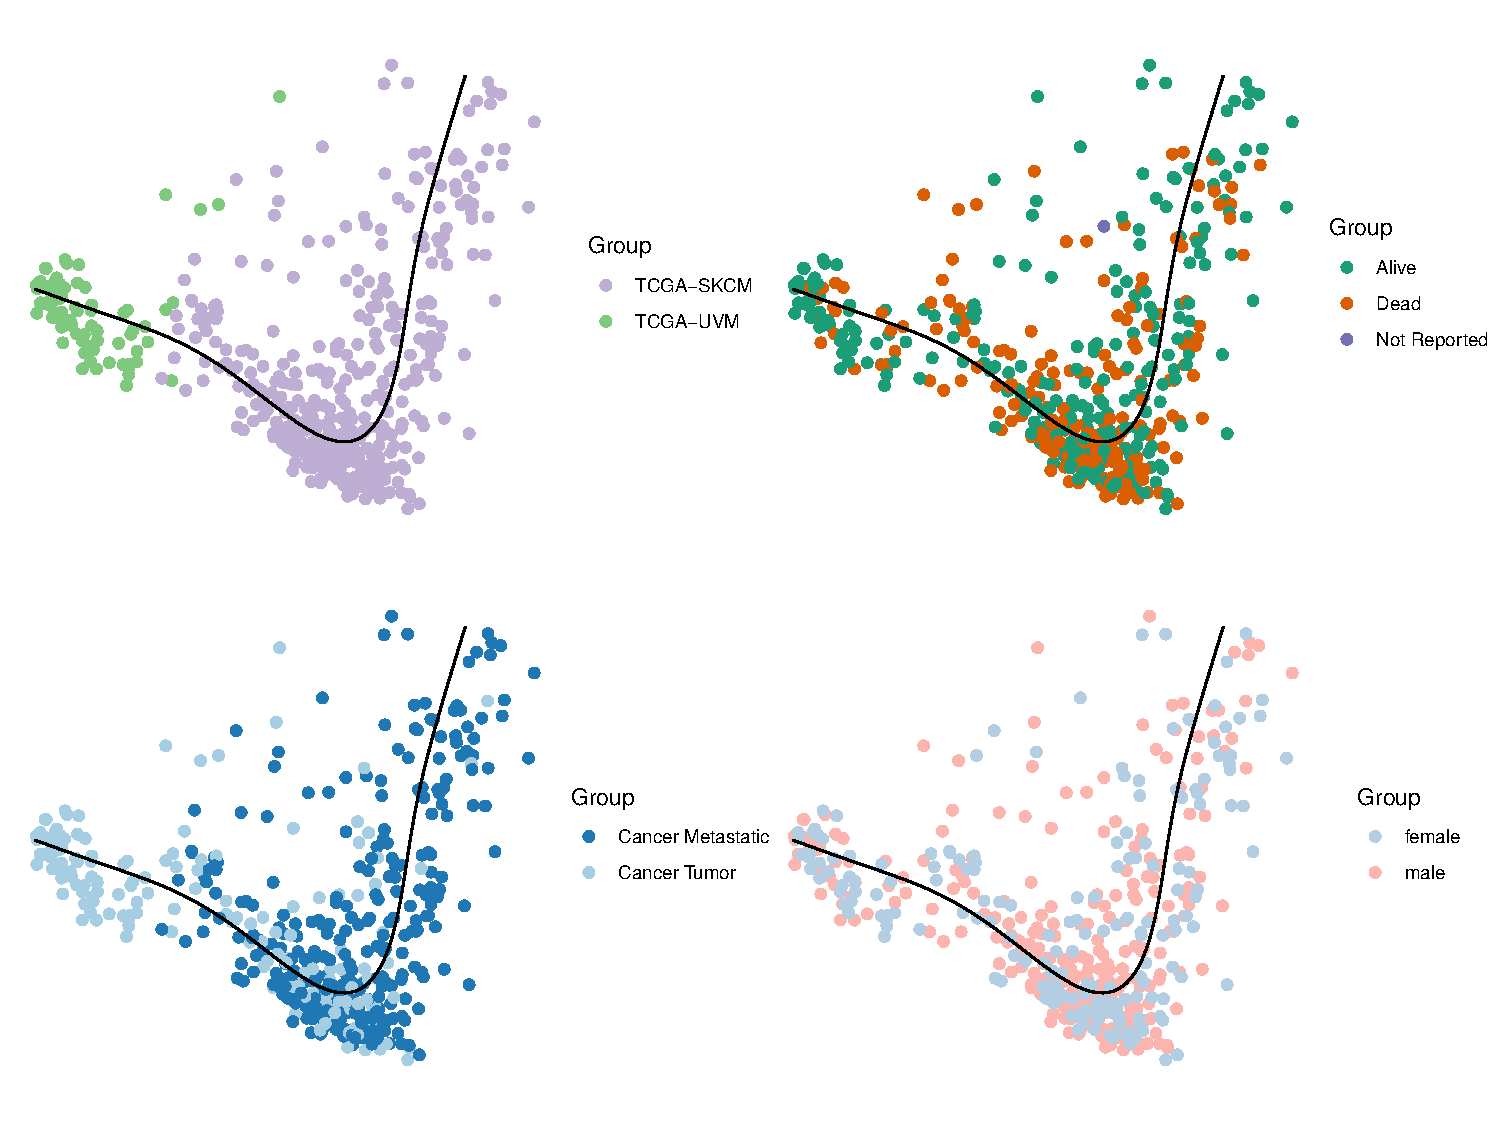
\includegraphics[width=.85\linewidth]{fig/tcga/zoom_cluster9_melanocytic-neoplasm_plot.pdf}\end{center}
	B
	\begin{center}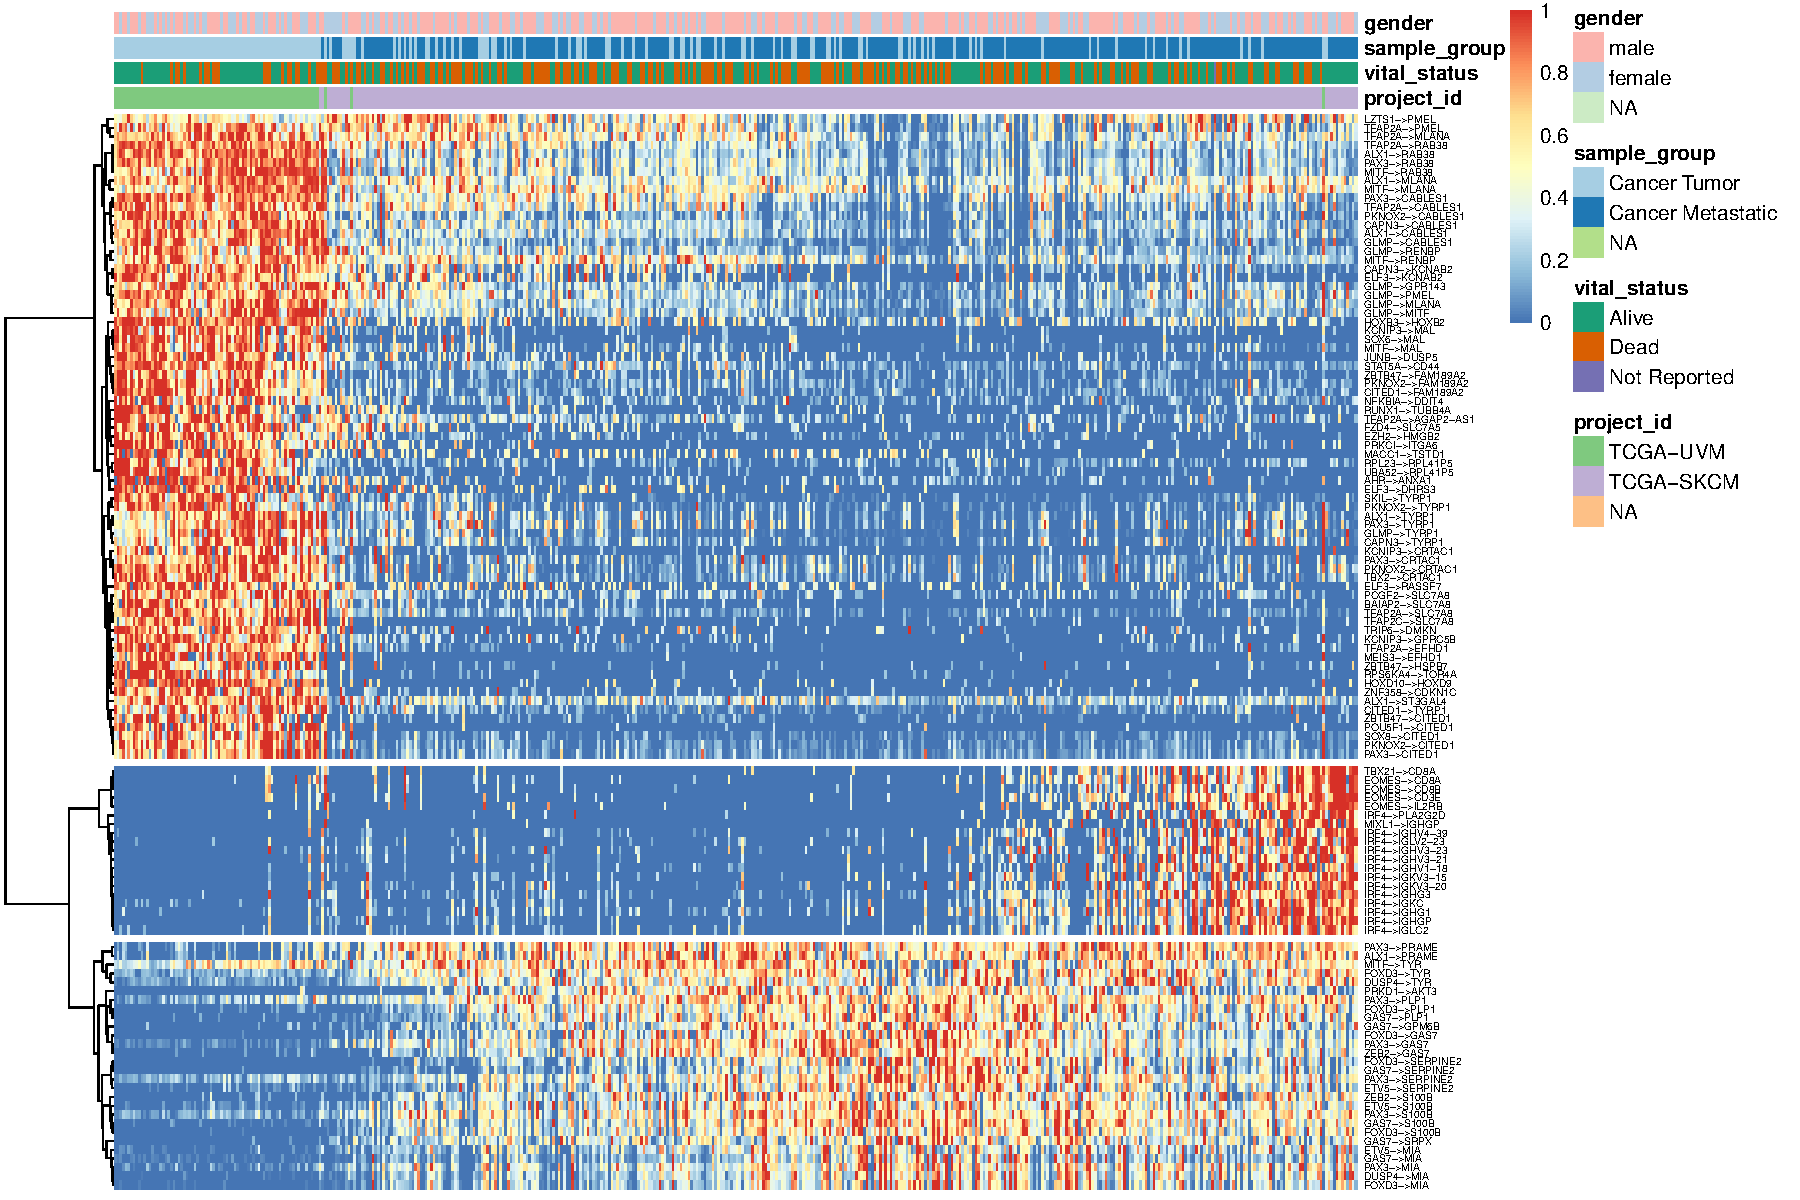
\includegraphics[width=.85\linewidth]{fig/tcga/zoom_cluster9_melanocytic-neoplasm_heatmap.pdf}\end{center}
	\caption{
		\textbf{In-depth view of cluster 9, melanocytic neoplasm.} 
		\textbf{A:} A dimensionality reduction of the samples, coloured according to multiple sources of meta-data. 
		\textbf{B:} The samples were ordered linearly with SCORPIUS (see trajectory in \textbf{A}) in order to visualise regulome activity in the form of a heatmap.
	}
	\label{fig:zoom9}
\end{figure}


\subsection{Kidney carcinoma}

\begin{figure}[H]
	A
	\begin{center}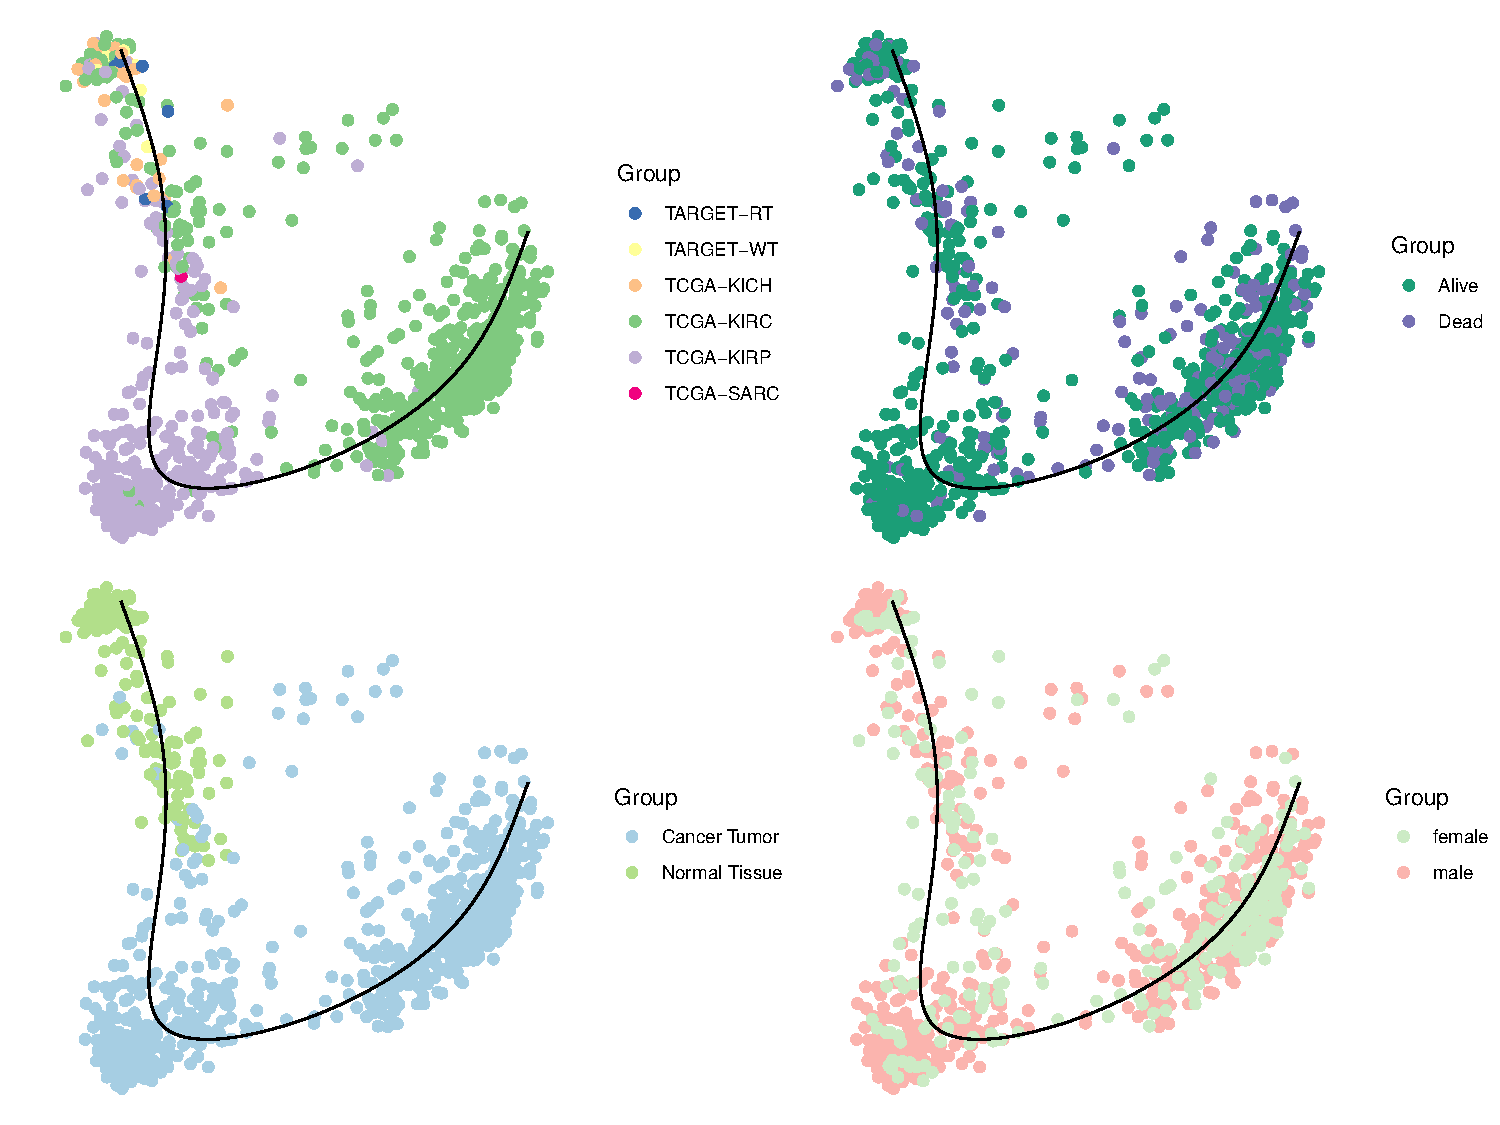
\includegraphics[width=.85\linewidth]{fig/tcga/zoom_cluster12_kidney-carcinoma_plot.pdf}\end{center}
	B
	\begin{center}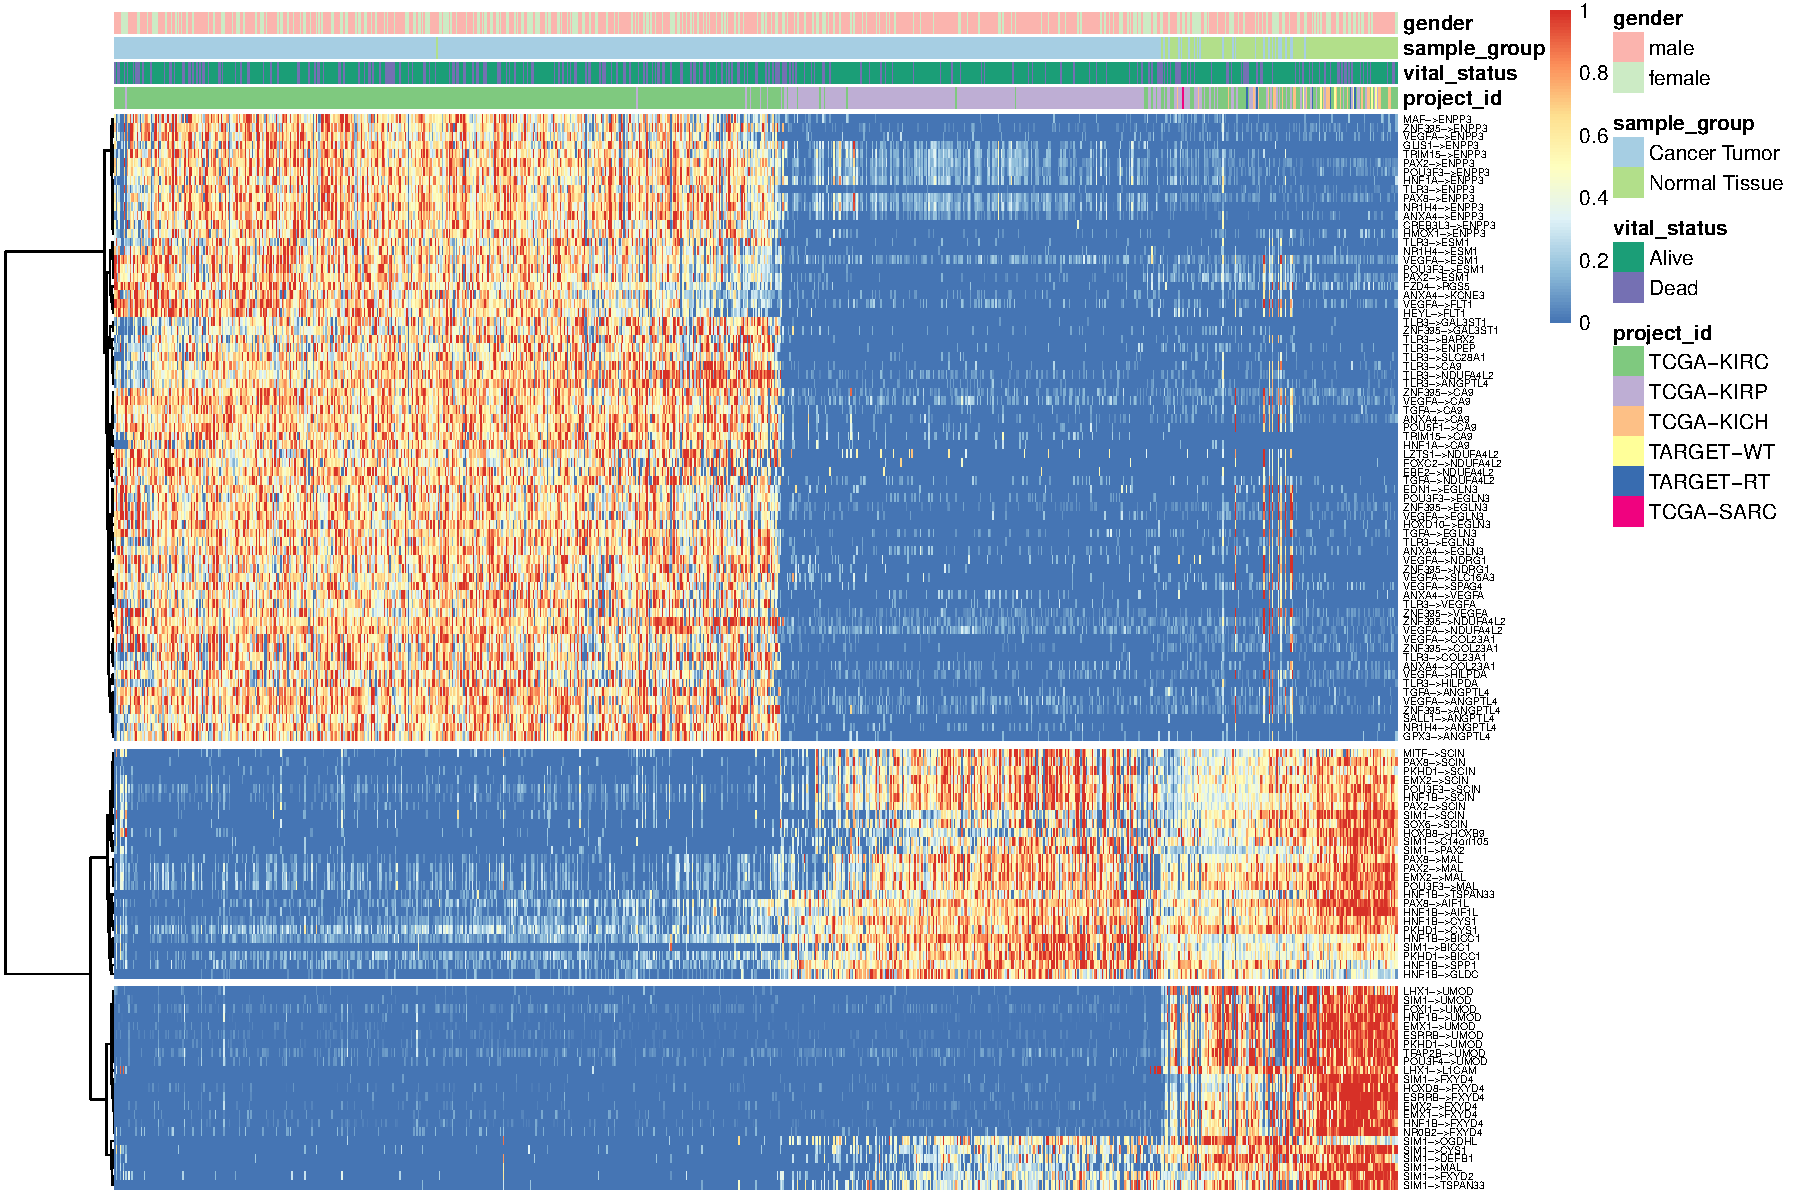
\includegraphics[width=.85\linewidth]{fig/tcga/zoom_cluster12_kidney-carcinoma_heatmap.pdf}\end{center}
	\caption{
		\textbf{In-depth view of cluster 12, kidney carcinoma.} 
		\textbf{A:} A dimensionality reduction of the samples, coloured according to multiple sources of meta-data. 
		\textbf{B:} The samples were ordered linearly with SCORPIUS (see trajectory in \textbf{A}) in order to visualise regulome activity in the form of a heatmap.
	}
	\label{fig:zoom12}
\end{figure}



\clearpage
\section{References}
\printbibliography[heading=none]
